\documentclass[aspectratio=169]{beamer}

\usetheme{metropolis}
\title{Лабораторная работа №3}
\subtitle{Набор математических формул в LaTeX}
\author{Николаев Дмитрий Иванович, НПМмд-02-24}
\institute{Российский университет дружбы народов имени Патриса Лумумбы}
\date{\today}

\usepackage[utf8]{inputenc}
\usepackage[russian]{babel}
\usepackage{graphicx}
\usepackage{listings}
\usepackage{xcolor}

\usepackage{amsmath}
\usepackage{bm}

\lstdefinestyle{mystyle}{
    backgroundcolor=\color{black!5},
    commentstyle=\color{green!40!black},
    keywordstyle=\color{magenta},
    stringstyle=\color{purple},
    basicstyle=\footnotesize\ttfamily,
    numbers=left,
    breaklines=true,
    numberstyle=\tiny\color{black!60},
    frame=tb,
    framerule=0pt,
}
\lstset{style=mystyle}

\begin{document}

\frame{\titlepage}

\section{Цели и задачи}
\begin{frame}{Цель работы}
    \begin{block}{Основная цель}
        Освоить базовые и расширенные средства LaTeX для набора математических формул: от простых внутристрочных выражений до сложных многострочных систем уравнений и матриц.
    \end{block}
    \begin{alertblock}{Ключевые задачи}
    \begin{itemize}
        \item Изучить базовые математические режимы и окружения.
        \item Освоить пакеты \texttt{amsmath}, \texttt{mathtools}, \texttt{bm} для продвинутой вёрстки.
        \item Научиться управлять стилями математических шрифтов.
        \item Попрактиковаться в создании перекрёстных ссылок на формулы.
    \end{itemize}
    \end{alertblock}
\end{frame}

\section{Выполнение работы}

\begin{frame}[fragile]{Часть 1: Основы математических режимов}
    \begin{columns}[T]
        \begin{column}{0.45\textwidth}
            \textbf{Ключевые примеры кода:}
            \begin{lstlisting}[language=tex]
\newcommand{\diff}{\mathop{}\!\mathrm{d}} % For upright
% Внутристрочный
$y = 2 \sin^2 \theta^{2}$

% Выключной
\[ \int_{-\infty}^{+\infty} e^{-x^2} dx \]

% Нумерованный
\begin{equation}
\int_{-\infty}^{+\infty} e^{-x^2} \diff x
\end{equation}
            \end{lstlisting}
        \end{column}
        \begin{column}{0.55\textwidth}
            \textbf{Результат:}
            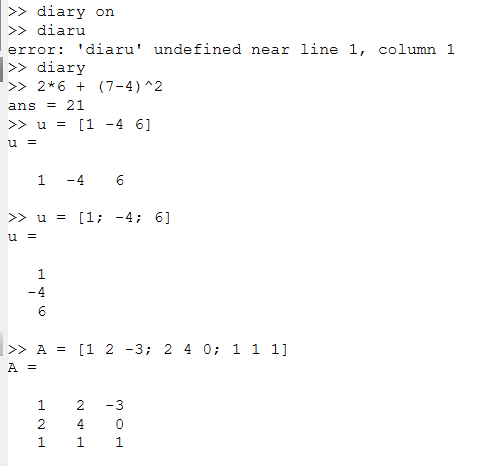
\includegraphics[width=\textwidth, height=0.7\textheight, keepaspectratio]{image/1.png}
        \end{column}
    \end{columns}
\end{frame}

\begin{frame}[fragile]{Часть 2: Пакет amsmath}
    \begin{columns}[T]
        \begin{column}{0.45\textwidth}
            \textbf{Выравнивание и матрицы:}
            \begin{lstlisting}[language=tex]
\begin{align*}
  Q_{n,0} &= 1 ... \\
  Q_{n,k} &= Q_{n-1,k}+Q_{n-1,k-1}+\binom{n}{k},
\end{align*}

\begin{pmatrix} % matrix; bmatrix
  a & b & c \\
  d & e & f
\end{pmatrix}
            \end{lstlisting}
        \end{column}
        \begin{column}{0.55\textwidth}
            \textbf{Результат:}
            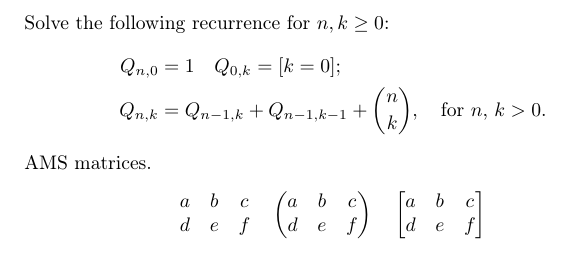
\includegraphics[width=\textwidth, height=0.7\textheight, keepaspectratio]{image/2.png}
        \end{column}
    \end{columns}
\end{frame}

\begin{frame}[fragile]{Часть 3: Стили шрифтов}
    \begin{columns}[T]
        \begin{column}{0.45\textwidth}
            \textbf{Код:}
            \begin{lstlisting}[language=tex]
The matrix $\mathbf{M}$ (for comparison $M$).

$\text{bad use } size \neq \mathit{size} \neq \mathrm{size} $

\textit{$\text{bad use } size \neq \mathit{size} \neq \mathrm{size} $}
            \end{lstlisting}
        \end{column}
        \begin{column}{0.55\textwidth}
            \textbf{Результат:}
            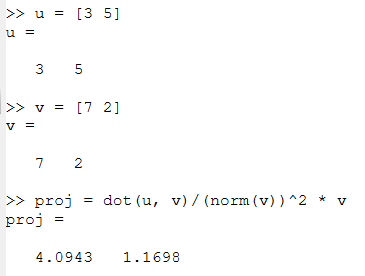
\includegraphics[width=\textwidth, height=0.7\textheight, keepaspectratio]{image/3.png}
        \end{column}
    \end{columns}
\end{frame}

\begin{frame}[fragile]{Часть 4: Многострочные формулы}
    \begin{columns}[T]
        \begin{column}{0.45\textwidth}
            \textbf{Ключевые окружения:}
            \begin{lstlisting}[language=tex]
% Группировка
\begin{gather} ... \end{gather}

% Длинная формула
\begin{multline*} ... \end{multline*}

% Колонки
\begin{align*}
 a &= b+1 & c &= d+2 ... \\
\end{align*}
            \end{lstlisting}
        \end{column}
        \begin{column}{0.55\textwidth}
            \textbf{Результат:}
            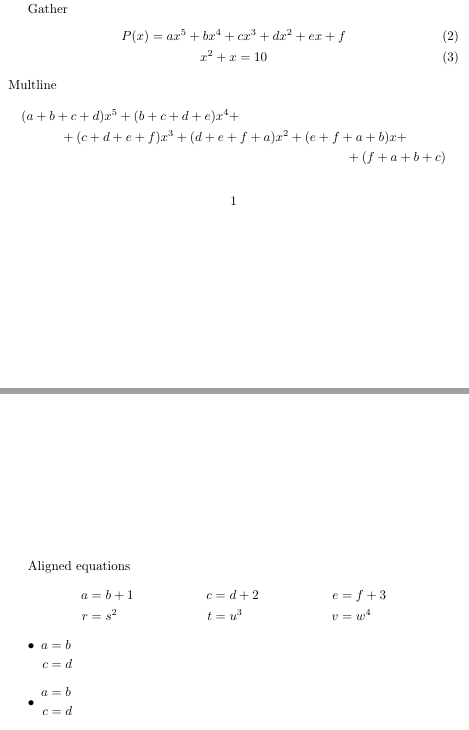
\includegraphics[width=\textwidth, height=0.7\textheight, keepaspectratio]{image/4.png}
        \end{column}
    \end{columns}
\end{frame}

\begin{frame}[fragile]{Части 5 и 6: Начертание и mathtools}
    \begin{columns}[T]
        \begin{column}{0.45\textwidth}
            \textbf{Сравнение \texttt{\textbackslash bm} и \texttt{\textbackslash mathbf}:}
            \begin{lstlisting}[language=tex]
% Не работает для греческих
$\mathbf{\pi} r^2$
% Работает для всего
$\alpha + \bm{\alpha}$
            \end{lstlisting}
            \textbf{Выравнивание в матрице:}
            \begin{lstlisting}[language=tex]
\begin{pmatrix*}[r]
  10000 & 11 \\ ...
\end{pmatrix*}
            \end{lstlisting}
        \end{column}
        \begin{column}{0.55\textwidth}
            \textbf{Результат:}
            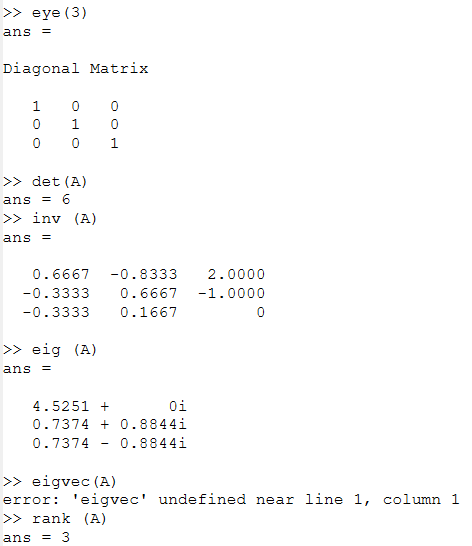
\includegraphics[width=\textwidth, height=0.7\textheight, keepaspectratio]{image/5.png}
        \end{column}
    \end{columns}
\end{frame}

\begin{frame}[fragile]{Часть 7: Специальные символы}
    \begin{columns}[T]
        \begin{column}{0.45\textwidth}
            \textbf{Разные начертания:}
            \begin{lstlisting}[language=tex]
One two three
\[
\log \alpha + \log \beta = \log(\alpha\beta)
\]

Unicode Math Alphanumerics
\[A + \symfrak{A}+\symbf{A}+ \symcal{A} + \symscr{A}+\symbb{A}\]

See~\eqref{eq_my}
\begin{equation}\label{eq_my}
\gamma + \symbf{\delta_{\symfrak{D}}^{\symcal{\varepsilon}}} = \symbb{DE}_{\symscr{\omega}}
\end{equation}
            \end{lstlisting}
        \end{column}
        \begin{column}{0.55\textwidth}
            \textbf{Результаты:}
            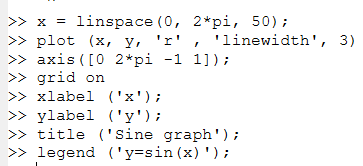
\includegraphics[width=\textwidth, keepaspectratio]{image/6.png}
            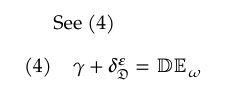
\includegraphics[width=\textwidth, keepaspectratio]{image/7.png}
        \end{column}
    \end{columns}
\end{frame}

\section{Итоговый результат}

\begin{frame}{Финальный документ}
    \begin{block}{Опции \texttt{fleqn} и \texttt{leqno}}
        В финальной версии документа опции класса \texttt{fleqn} и \texttt{leqno} выравнивают все выключные формулы и их нумерацию по левому краю.
    \end{block}
    \begin{columns}[T]
        \begin{column}{0.5\textwidth}
            \textbf{Результат (начало документа):}
            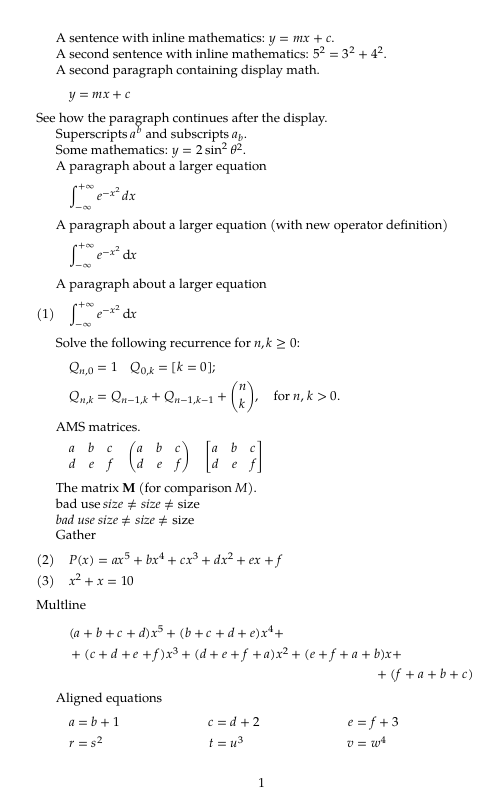
\includegraphics[width=\textwidth, height=0.6\textheight, keepaspectratio]{image/8_1.png}
        \end{column}
        \begin{column}{0.5\textwidth}
            \textbf{Результат (конец документа):}
            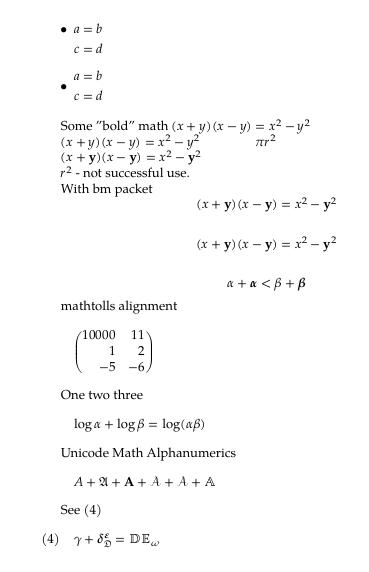
\includegraphics[width=\textwidth, height=0.6\textheight, keepaspectratio]{image/8_2.png}
        \end{column}
    \end{columns}
\end{frame}

\begin{lstlisting}[
    %float=htbp, 
    %allowpagebreak,
    language=tex,
    caption={Полный исходный код файла lab3.tex}, 
    label=lst:final_code
]
\documentclass[fleqn,leqno]{article}
\usepackage[T1]{fontenc}
\usepackage{amsmath}
\usepackage{bm}
\usepackage{mathtools}

\usepackage{unicode-math}
\setmainfont{TeX Gyre Pagella}
\setmathfont{TeX Gyre Pagella Math}
%\newcommand{\diff}{\mathop{}\!d} % For italic
\newcommand{\diff}{\mathop{}\!\mathrm{d}} % For upright

\begin{document}

A sentence with inline mathematics: \(y = mx + c\).

A second sentence with inline mathematics:
$5^{2}=3^{2}+4^{2}$.

A second paragraph containing display math.
\[
y = mx + c
\]
See how the paragraph continues after the display.

Superscripts $a^{b}$ and subscripts $a_{b}$.

Some mathematics: $y = 2 \sin^2 \theta^{2}$.

A paragraph about a larger equation
\[
\int_{-\infty}^{+\infty} e^{-x^2} \, dx
\]

A paragraph about a larger equation (with new operator definition)
\[
\int_{-\infty}^{+\infty} e^{-x^2} \diff x
\]

A paragraph about a larger equation
\begin{equation}
\int_{-\infty}^{+\infty} e^{-x^2} \diff x
\end{equation}

%------------------------------

Solve the following recurrence for $ n,k\geq 0 $:
\begin{align*}
Q_{n,0} &= 1 \quad Q_{0,k} = [k=0]; \\
Q_{n,k} &= Q_{n-1,k}+Q_{n-1,k-1}+\binom{n}{k},
\quad\text{for $n$, $k>0$.}
\end{align*}

AMS matrices.
\[
\begin{matrix}
a & b & c \\
d & e & f
\end{matrix}
\quad
\begin{pmatrix}
a & b & c \\
d & e & f
\end{pmatrix}
\quad
\begin{bmatrix}
a & b & c \\
d & e & f
\end{bmatrix}
\]

%---------------------------------

The matrix $\mathbf{M}$ (for comparison $M$).

$\text{bad use } size \neq \mathit{size} \neq \mathrm{size} $

\textit{$\text{bad use } size \neq \mathit{size} \neq
\mathrm{size} $}

%---------------------------------

Gather
\begin{gather}
P(x)=ax^{5}+bx^{4}+cx^{3}+dx^{2}+ex +f\\
x^2+x=10
\end{gather}
Multline
\begin{multline*}
(a+b+c+d)x^{5}+(b+c+d+e)x^{4} + \\
+(c+d+e+f)x^{3}+(d+e+f+a)x^{2}+(e+f+a+b)x + \\
+ (f+a+b+c)
\end{multline*}

Aligned equations
\begin{align*}
a &= b+1 & c &= d+2 & e &= f+3 \\
r &= s^{2} & t &=u^{3} & v &= w^{4}
\end{align*}

\begin{itemize}
\item
$\begin{aligned}[t]
a&=b\\
c&=d
\end{aligned}$
\item
$\begin{aligned}
a&=b\\
c&=d
\end{aligned}$
\end{itemize}

%---------------------------------

Some "bold" math
$(x+y)(x-y)=x^{2}-y^{2}$

{\boldmath $(x+y)(x-y)=x^{2}-y^{2}$ $\qquad \qquad \pi r^2$}

$(x+\mathbf{y})(x-\mathbf{y})=x^{2}-{\mathbf{y}}^{2}$

$\mathbf{\pi} r^2$ - not successful use. % bad use of \mathbf

With bm packet
$$(x+\mathbf{y})(x-\mathbf{y})=x^{2}-{\mathbf{y}}^{2}$$

$$(x+\symbf{y})(x-\symbf{y}) \symbf{=} x^{2}-{\symbf{y}}^{2}$$

$$\alpha + \symbf{\alpha} < \beta + \symbf{\beta}$$

%---------------------------------

mathtolls alignment
\[
\begin{pmatrix*}[r]
10000&11\\
1&2\\
-5&-6
\end{pmatrix*}
\]

%---------------------------------

One two three
\[
\log \alpha + \log \beta = \log(\alpha\beta)
\]

Unicode Math Alphanumerics
\[A + \symfrak{A}+\symbf{A}+ \symcal{A} + \symscr{A}+\symbb{A}\]


%---------------------------------

See~\eqref{eq_my}
\begin{equation}\label{eq_my}
\gamma + \symbf{\delta_{\symfrak{D}}^{\symcal{\varepsilon}}} = \symbb{DE}_{\symscr{\omega}}
\end{equation}

\end{document}
\end{lstlisting}

\section{Выводы}

\begin{frame}{Выводы}
    \begin{alertblock}{Освоенные навыки}
    \begin{itemize}
        \item Применение базовых математических режимов и окружений.
        \item Использование продвинутых пакетов: \texttt{amsmath}, \texttt{mathtools}, \texttt{bm}.
        \item Вёрстка сложных многострочных и многоколончатых уравнений.
        \item Управление стилями и начертанием математических символов.
        \item Изменение глобального форматирования формул с помощью опций класса документа.
    \end{itemize}
    \end{alertblock}
\end{frame}

\end{document}